%%%%%%%%%%%%%%%%%%%%%%%%%%%%%%%%%%%%%%%%%%%%%%%%%%%%%%%%%%%%%%%%%%%%%%%%%%%
%
% Template for a LaTex article.
%
%%%%%%%%%%%%%%%%%%%%%%%%%%%%%%%%%%%%%%%%%%%%%%%%%%%%%%%%%%%%%%%%%%%%%%%%%%%

\documentclass[12pt,a4paper]{article}
\usepackage{graphicx}
\usepackage[utf8]{inputenc}
\usepackage[T1]{fontenc}
\usepackage[english]{babel}
%\usepackage[spanish]{babel}
\usepackage{tikz}

% AMS packages:
\usepackage{amsmath, amsthm, amsfonts}

\usepackage{algpseudocode}
\usepackage{algorithm}
%\usepackage[skip, parfill]{parskip}
%\usepackage{parskip}


% Theorems
%-----------------------------------------------------------------
\newtheorem{thm}{Theorem}[section]
\newtheorem{cor}[thm]{Corollary}
\newtheorem{lem}[thm]{Lemma}
\newtheorem{prop}[thm]{Proposition}
\theoremstyle{definition}
\newtheorem{defn}[thm]{Definition}
\theoremstyle{remark}
\newtheorem{rem}[thm]{Remark}

% Shortcuts.
% One can define new commands to shorten frequently used
% constructions. As an example, this defines the R and Z used
% for the real and integer numbers.
%-----------------------------------------------------------------
\def\RR{\mathbb{R}}
\def\ZZ{\mathbb{Z}}
\def\QQ{\mathbb{Q}}
\def\NN{\mathbb{N}}

% Similarly, one can define commands that take arguments. In this
% example we define a command for the absolute value.
% -----------------------------------------------------------------
\newcommand{\abs}[1]{\left\vert#1\right\vert}

% Operators
% New operators must defined as such to have them typeset
% correctly. As an example we define the Jacobian:
% -----------------------------------------------------------------
\DeclareMathOperator{\Jac}{Jac}
% This makes the same as \DeclareMathOperator{\Jac}{Jac}
% \newcommand{\Jac}{\operatorname{Jac}}
\DeclareMathOperator{\Ker}{Ker}
\DeclareMathOperator{\Max}{Max}
\DeclareMathOperator{\End}{End}

%-----------------------------------------------------------------
\title{Template for a \LaTeX\ article}
\author{Angela Menéndez\\
  \small A-level, Year 12D\\
  \small TEMS\\
  \small Madrid
}

%\setlength{\parindent}{0em}
%\setlength{\parskip}{0.5em}
%\renewcommand{\baselinestretch}{1}

\begin{document}

\maketitle



%\abstract{
%This is a simple template for an article written in \LaTeX, with a few useful examples as introduction to \LaTeX environment.}

%\setlength{\parindent}{0em}
%\setlength{\parskip}{0.5em}

\bigskip 
\begin{center}
\textbf{Fake Abstract}
\end{center}

This is a simple template for an article written in \LaTeX, with a few useful examples as introduction to pdflatex environment.This is a simple template for an article written in latex, with a few useful examples as introduction to pdflatex environment.

This is a simple template for an article written in \LaTeX, with a few useful examples as introduction to \LaTeX environment.


\section{Section for some maths typing examples}\label{sec:maths_examples}

Here goes the text of this first section.

In this section a few examples of the use of 
\verb|\DeclareMathOperator| will we put in practice.


The \LaTeX code:

\begin{center}
\begin{verbatim}
\begin{displaymath}
  \Max_{x\in A} f(x) \qquad  \End_R V 
\end{displaymath}
\end{verbatim}
\end{center}

Produces:
\begin{displaymath}
  \Max_{x\in A} f(x) \qquad  \End_R V 
\end{displaymath}


\begin{equation}\label{eq:area}
  S = \pi r^2
\end{equation}
\[S_n = \sum_{n=1}^{\infty} \frac{1}{n^3} + \sum_{n=1}^{\infty} \frac{1}{n^3}\] 

One can refer to equations like this: see equation (\ref{eq:area}). One can also
refer to sections in the same way: see section \ref{sec:pictures_graphs}. Or
to the bibliography like this: \cite{Cd94}.

One can refer to equations like this: see equation (\ref{eq:area}). One can also
refer to sections in the same way: see section \ref{sec:pictures_graphs}. Or
to the bibliography like this: \cite{Cd94}.

More text. Claro 
\[\RR\ \text{is the set of real numbers}\]
\[\ZZ\ \text{is the set of integer numbers}\]



\subsection{Subsection}\label{sec:nothing}

\section{pseudo code}\label{sec:pseudo_code}

This is my first algorithm with \LaTeX

\begin{algorithmic}[1]
\State $i \gets 10$
\If{$i\geq 5$} 
    \State $i \gets i-1$
\Else
    \If{$i\leq 3$}
        \State $i \gets i+2$
    \EndIf
\EndIf 
\end{algorithmic}

\bigskip 
And next is the second
\begin{algorithmic}
\Require $n \geq 0$
\Ensure $y = x^n$
\State $y \gets 1$
\State $X \gets x$
\State $N \gets n$
\While{$N \neq 0$}
\If{$N$ is even}
    \State $X \gets X \times X$
    \State $N \gets \frac{N}{2}$  \Comment{This is a comment}
\ElsIf{$N$ is odd}
    \State $y \gets y \times X$
    \State $N \gets N - 1$
\EndIf
\EndWhile
\end{algorithmic}



The complete pseudo code with titles:

\begin{algorithm}
\caption{An algorithm with caption}\label{alg:cap}
\begin{algorithmic}[1]
\Require $n \geq 0$
\Ensure $y = x^n$
\State $y \gets 1$
\State $X \gets x$
\State $N \gets n$
\While{$N \neq 0$}
\If{$N$ is even}
    \State $X \gets X \times X$
    \State $N \gets \frac{N}{2}$  \Comment{This is a comment}
\ElsIf{$N$ is odd}
    \State $y \gets y \times X$
    \State $N \gets N - 1$
\EndIf
\EndWhile
\end{algorithmic}
\end{algorithm}



\section{Pictures and graphs}\label{sec:pictures_graphs}

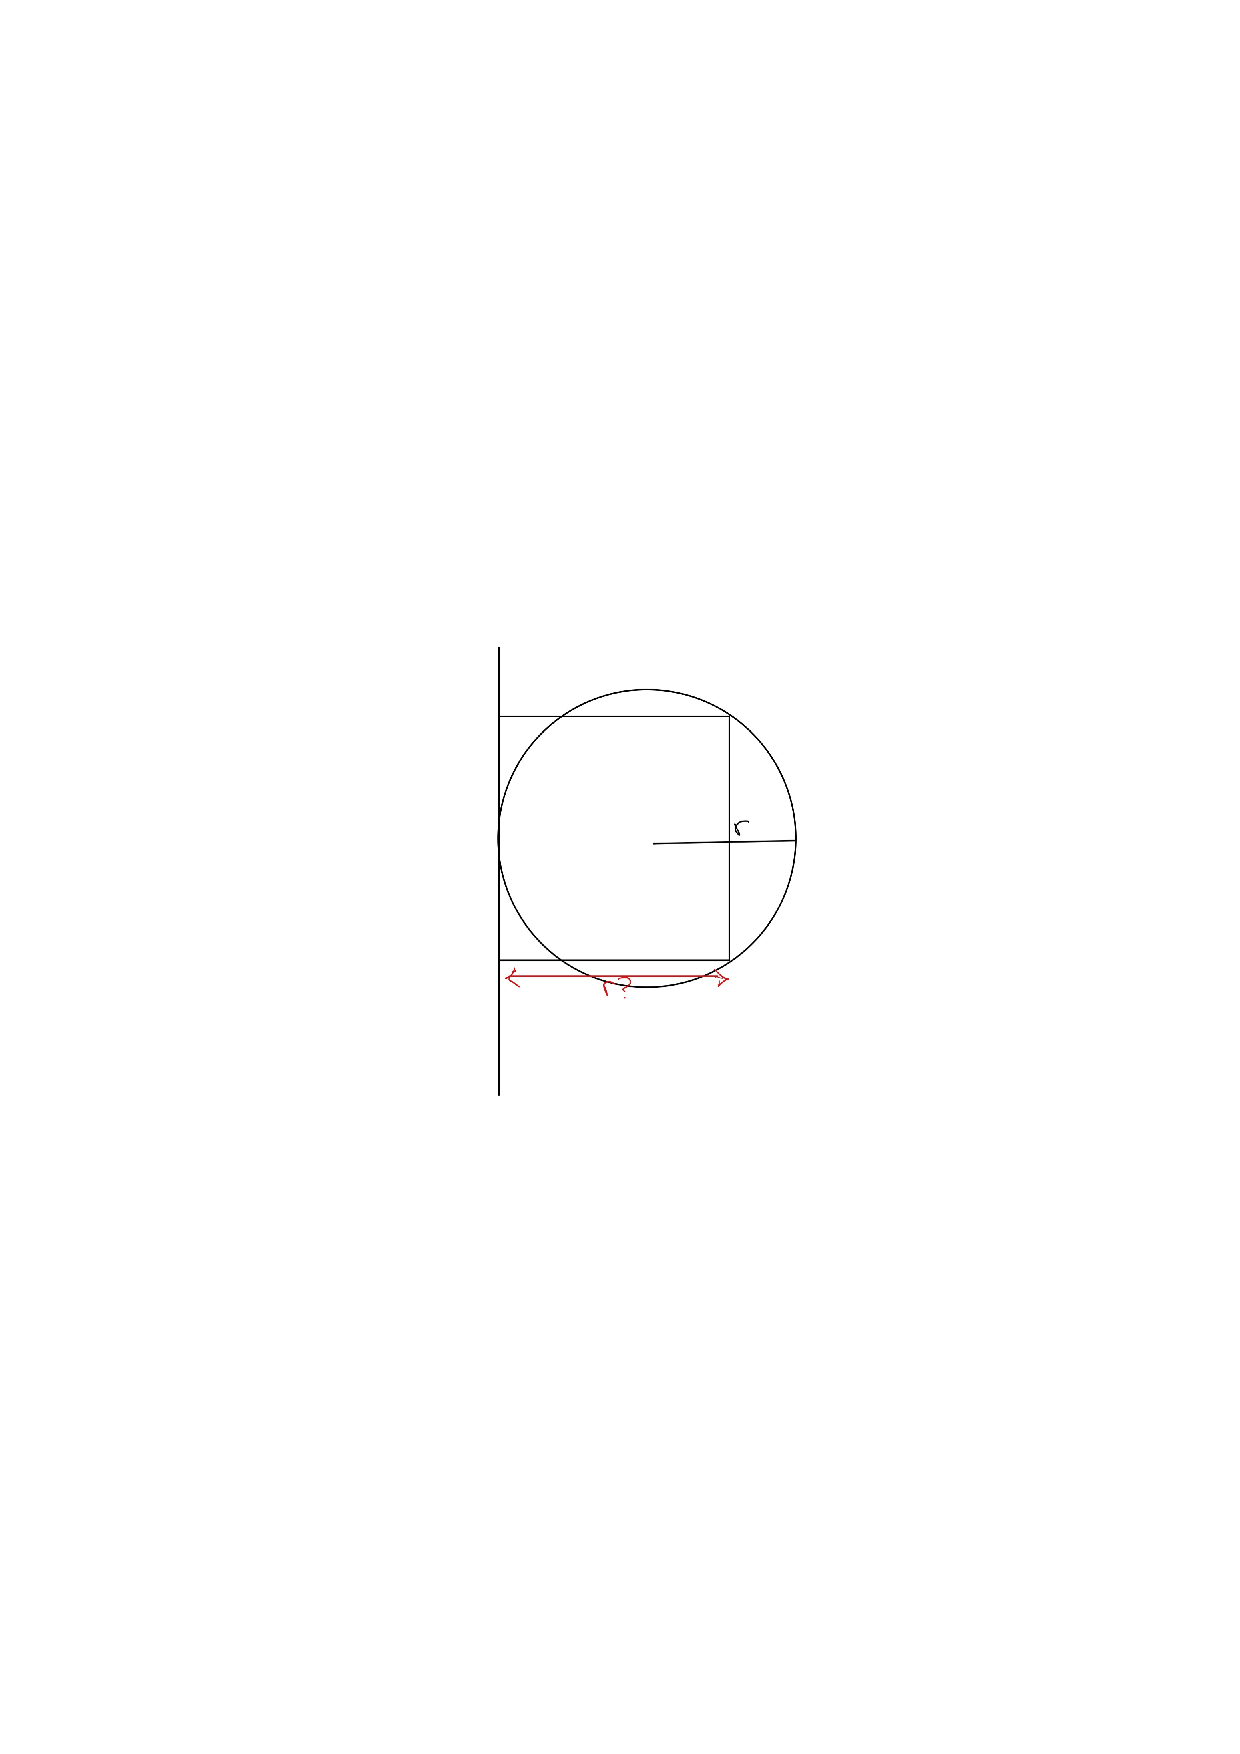
\includegraphics[width=0.6\textwidth]{./figs/radius_scure.jpg}

\subsubsection{Subsubsection}\label{sec:nothing2}

More text \cite{Someone2000}


\includegraphics[width=0.8\textwidth]{./figs/latex_logo.png}


\section{LaTeX Graphics using TikZ}

\bigskip 
\begin{center}
\begin{tikzpicture}
\draw (0,0) -- (8,0) -- (8,8) -- (0,8) -- (0,0);
\end{tikzpicture}
\end{center}


\bigskip 
\begin{tikzpicture}
\draw (0,0) -- (8,0) -- (8,8) -- cycle;
\draw (0,0) parabola (-4,8);
\end{tikzpicture}

\bigskip 
\begin{tikzpicture}
\draw (0,0) .. controls (0,10) and (10,0) .. (10,10);
\end{tikzpicture}


\bigskip 
\begin{tikzpicture}
\draw (0,0) -- (1,0) -- (1,1) -- (0,1) -- (0,0);
\draw[red,thick,dashed] (3,3) circle (4cm);
\end{tikzpicture}

\bigskip 
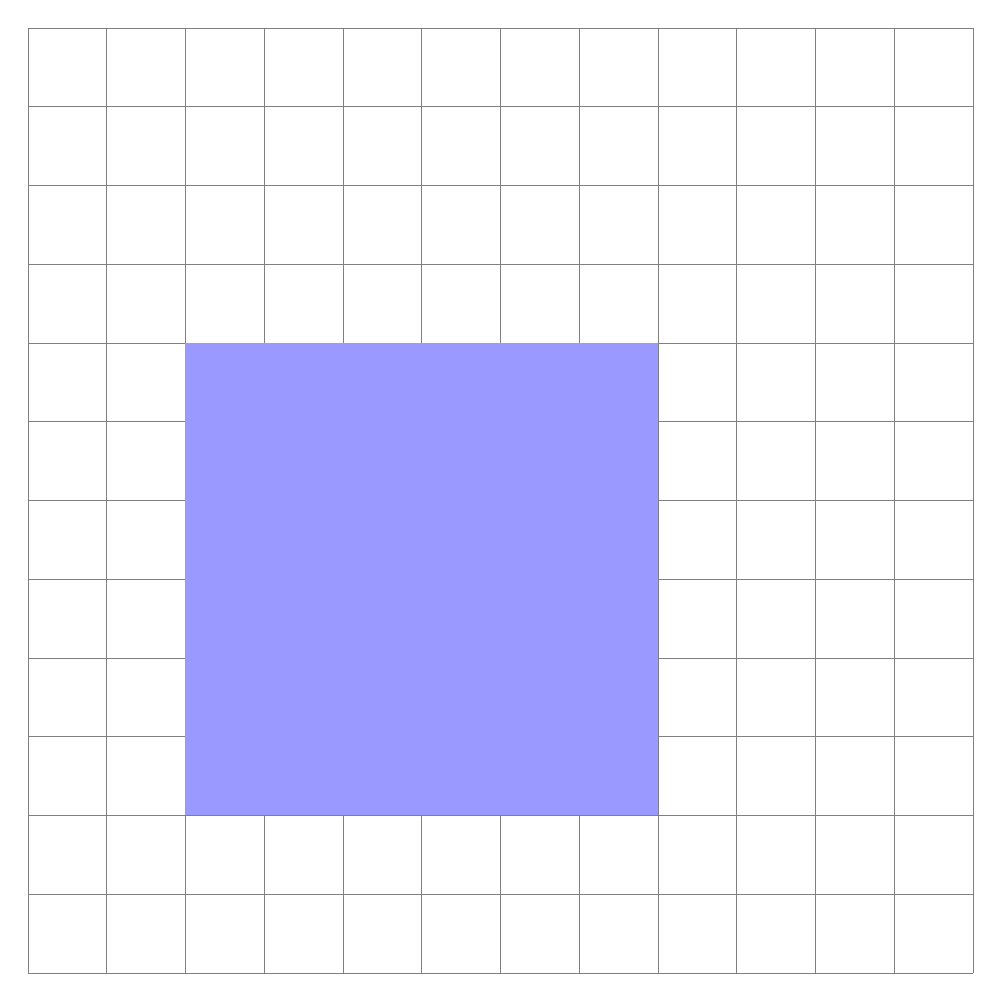
\begin{tikzpicture}
\draw[step=1cm,gray,very thin] (-2,-2) grid (10,10);
\fill[blue!40!white] (0,0) rectangle (6,6);
\end{tikzpicture}

\bigskip 
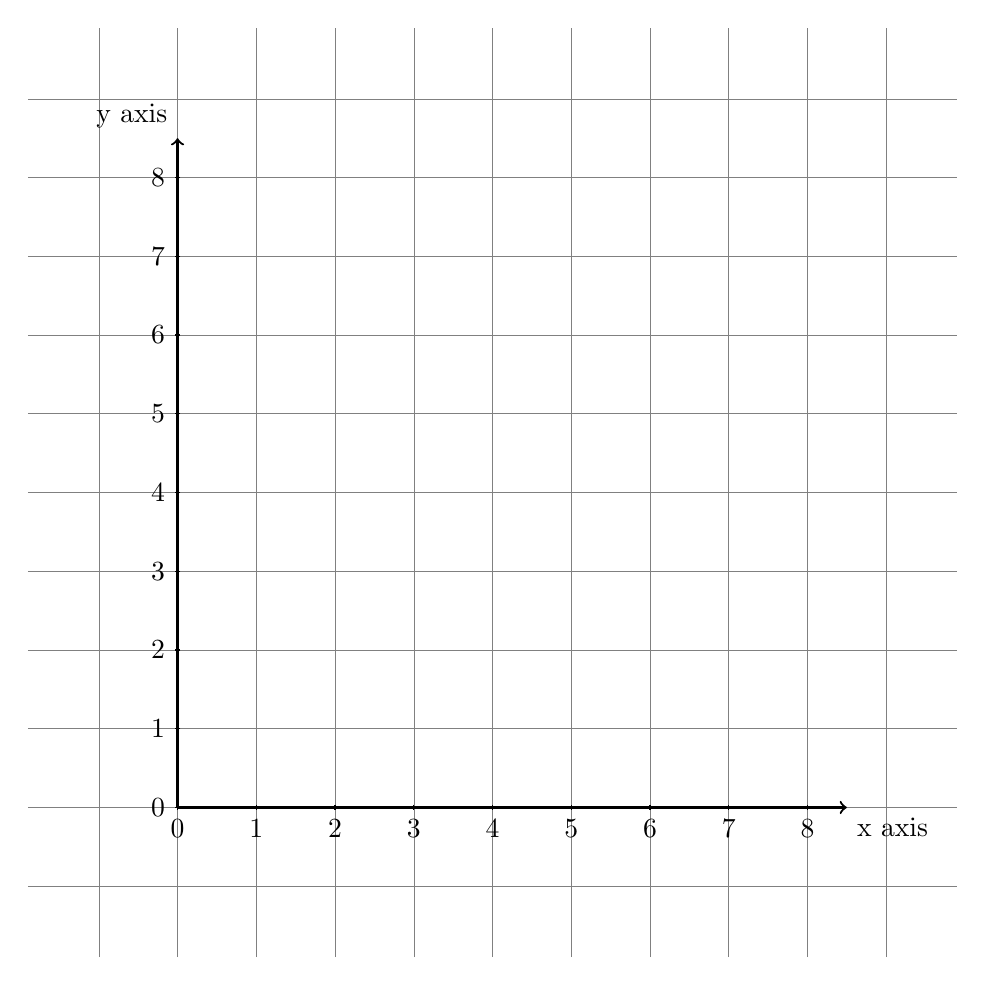
\begin{tikzpicture}
\draw[step=1cm,gray,very thin] (-1.9,-1.9) grid (9.9,9.9);
\draw[thick,->] (0,0) -- (8.5,0) node[anchor=north west] {x axis};
\draw[thick,->] (0,0) -- (0,8.5) node[anchor=south east] {y axis};

\foreach \x in {0,1,2,3,4,5,6,7,8}
   \draw (\x cm,1pt) -- (\x cm,-1pt) node[anchor=north] {$\x$};
\foreach \y in {0,1,2,3,4,5,6,7,8}
    \draw (1pt,\y cm) -- (-1pt,\y cm) node[anchor=east] {$\y$};
    
\end{tikzpicture}


\newpage
% Bibliography
%-----------------------------------------------------------------
\begin{thebibliography}{99}

\bibitem{Cd94} 
	Author,
	\emph{Title}
	\newblock{Journal/Editor, (year)}


\bibitem{Author1990}
    A.~Author.
    \newblock {\em Handbook of Everything}.
    \newblock Some Press, 1990.

  \bibitem{Someone2000}
    S.~Someone.
    \newblock On this and that.
    \newblock {\em Journal of This and That}, 2(1):50--100,
    2000.
\end{thebibliography}


\end{document}
